\documentclass[10pt,twocolumn]{article}
\usepackage[margin=0.75in]{geometry}
\usepackage{amsmath,amssymb,amsfonts,amsthm}
\usepackage{graphicx}
\bibliographystyle{plain}
\raggedbottom
\renewcommand{\arraystretch}{1.15}
\newcommand{\toprule}{\hline\hline}
\newcommand{\midrule}{\hline}
\newcommand{\bottomrule}{\hline\hline}
\newcommand{\citep}[1]{\cite{#1}}
\newcommand{\citet}[1]{\cite{#1}}

\newtheorem{proposition}{Proposition}
\newtheorem{remark}{Remark}

\title{\textbf{Quaternion-Tucker ZigZag Networks: Halving Transformer Backbone Parameters via Shared Hypercomplex Tensor Cores and Braided Top-Down Routing}}
\author{
    \textbf{Shubham Barmase} \\
    \small Independent Researcher
}
\date{November 2026}

\begin{document}
\maketitle

\section*{Abstract}
\noindent Standard Transformer architectures allocate independent, dense two-dimensional weight matrices to every feed-forward network (FFN) layer, coupling parameter count linearly with depth ($O(L)$). Conversely, weight-tied Looped Transformers and Deep Equilibrium Models decouple depth from parameters ($O(1)$) but enforce time-homogeneous updates across iterations, limiting depth-specific specialization. In this work, we formulate the entire $L$-layer FFN stack as a unified \textbf{3D Tensor Cuboid} $\mathcal{W} \in \mathbb{R}^{L \times d \times d}$ and introduce \textbf{QuatTucker-ZigZagGPT}, an architecture unifying three orthogonal mechanisms: (1) \textbf{4D Quaternion Hamilton Algebra ($\mathbb{H}$)} for hypercomplex feature projections compiled into a single fused \texttt{bfloat16} Tensor-Core GEMM ($4\times$ FFN compression), (2) \textbf{Block-Diagonal Tucker SwiGLU Cores} that allow each depth slice to execute distinct $64 \times 64$ subspace rotations over a single shared high-rank feature basis, and (3) \textbf{Braided ZigZag Diamond Routing} ($L_0 \to L_2 \to L_1(h_0 + h_2) \to L_3(h_1 + h_2)$), which introduces zero-FLOP, zero-parameter coarse-to-fine top-down refinement. We further introduce \textbf{Annealed Gated Bounce-Back Scaffolding (\texttt{GatedBounce})}, a sparsity-taxed training-time feedback path that self-distills to $0.0\%$ inference overhead. Across six empirical domains---8-bit Parity, Mod-53 Algorithmic Grokking, Handwritten Digits, 3-Turn Intertwined Spirals, TinyStories, and GPT-2 BPE pretraining on \texttt{FineWeb-Edu}---our architectures consistently match or outperform standard ResNets and FlashAttention Transformers at $2\times$--$7.6\times$ parameter compression. On \texttt{FineWeb-Edu} (11.4M train / 600k val tokens, NVIDIA L4), \textbf{QuatTucker-ZigZagGPT-8} (26.5M total / \textbf{7.2M backbone} parameters) achieves \textbf{5.1339 validation loss (169.68 PPL)}, outperforming a 33.5M (\textbf{14.3M backbone}) FlashAttention \texttt{StandardGPT-8} baseline (5.2310 loss / 186.98 PPL) by $-0.0971$ loss ($-17.30$ PPL) with \textbf{half the backbone parameters} and monotonic validation descent through step 3,000.

\section{Introduction}
The dominant scaling paradigm in deep learning relies on stacking $L$ sequential, independent layers of dense two-dimensional weight matrices \citep{vaswani2017attention}. In modern Large Language Models (LLMs), feed-forward networks (FFNs) typically account for two-thirds of all non-embedding parameters, binding memory bandwidth and VRAM capacity linearly to depth.

Weight-tied recurrent architectures---such as Universal Transformers \citep{dehghani2019universal}, Deep Equilibrium Models (DEQs) \citep{bai2019deep}, and Looped Transformers \citep{giannou2023looped}---decouple parameter count from compute depth by iterating a single block $T$ times. However, strict weight-tying imposes a \emph{time-homogeneous} dynamical system ($h_{t+1} = f_W(h_t)$), forcing every depth step to share an identical transformation. Simultaneously, tensor decomposition methods \citep{kolda2009tensor, novikov2015tensorizing} and hypercomplex Quaternion networks \citep{parcollet2019quaternion, tay2019lightweight} have demonstrated strong parameter compression, yet rarely integrate cleanly with modern fused \texttt{bfloat16} GPU Tensor Cores and FlashAttention \citep{dao2022flashattention}.

In this paper, we bridge looped recurrence, tensor decomposition, hypercomplex algebra, and non-sequential top-down routing into a unified, GPU-native architecture. Our investigation proceeds from first-principles algorithmic benchmarks to 33.5M-parameter BPE language modeling, yielding both positive breakthroughs and sharp negative falsifications:
\begin{itemize}
    \item \textbf{Annealed Gated Bounce-Back Scaffolding (\texttt{GatedBounce}):} A conditional feedback gate to $L_1$ penalized by a sparsity tax $\lambda$. Under strong $\lambda=0.2$, the network uses bounce-back as early-epoch scaffolding and self-distills the algorithm into plain feedforward weights, lifting 8-bit Parity generalization from $62.2\%$ to $90.9\%$ at $0.0\%$ inference overhead.
    \item \textbf{Braided \texttt{ZigZag} Diamond Routing:} Reordering 4-layer blocks into $L_0 \to L_2 \to L_1(h_0+h_2) \to L_3(h_1+h_2)$ creates a coarse-to-fine top-down diamond with zero extra FLOPs or parameters, slashing parity variance by $3.6\times$ and improving \texttt{TinyStories} perplexity.
    \item \textbf{Block-Diagonal Tucker SwiGLU \& 4D Quaternion Algebra ($\mathbb{H}$):} Treating the 4-layer FFN stack as a shared 3D tensor cuboid factorized via 4D Quaternions and specialized per depth via a real-valued $64 \times 64$ Tucker core cuts the 8-layer Transformer backbone in half ($7.2\text{M}$ vs.\ $14.3\text{M}$) while beating \texttt{StandardGPT-8} by $-17.30$ PPL on \texttt{FineWeb-Edu}.
    \item \textbf{Architectural Boundaries (Negative Results):} We empirically falsify shared CP-decomposed attention (\texttt{FullTucker-ZigZagGPT-12}), complex FFT/cuFFT rank mixing, and periodic phase-gated backprop valves, establishing that \emph{attention must remain dense and independent per layer while FFNs thrive under hypercomplex tensor sharing}.
\end{itemize}

\begin{figure*}[t]
    \centering
    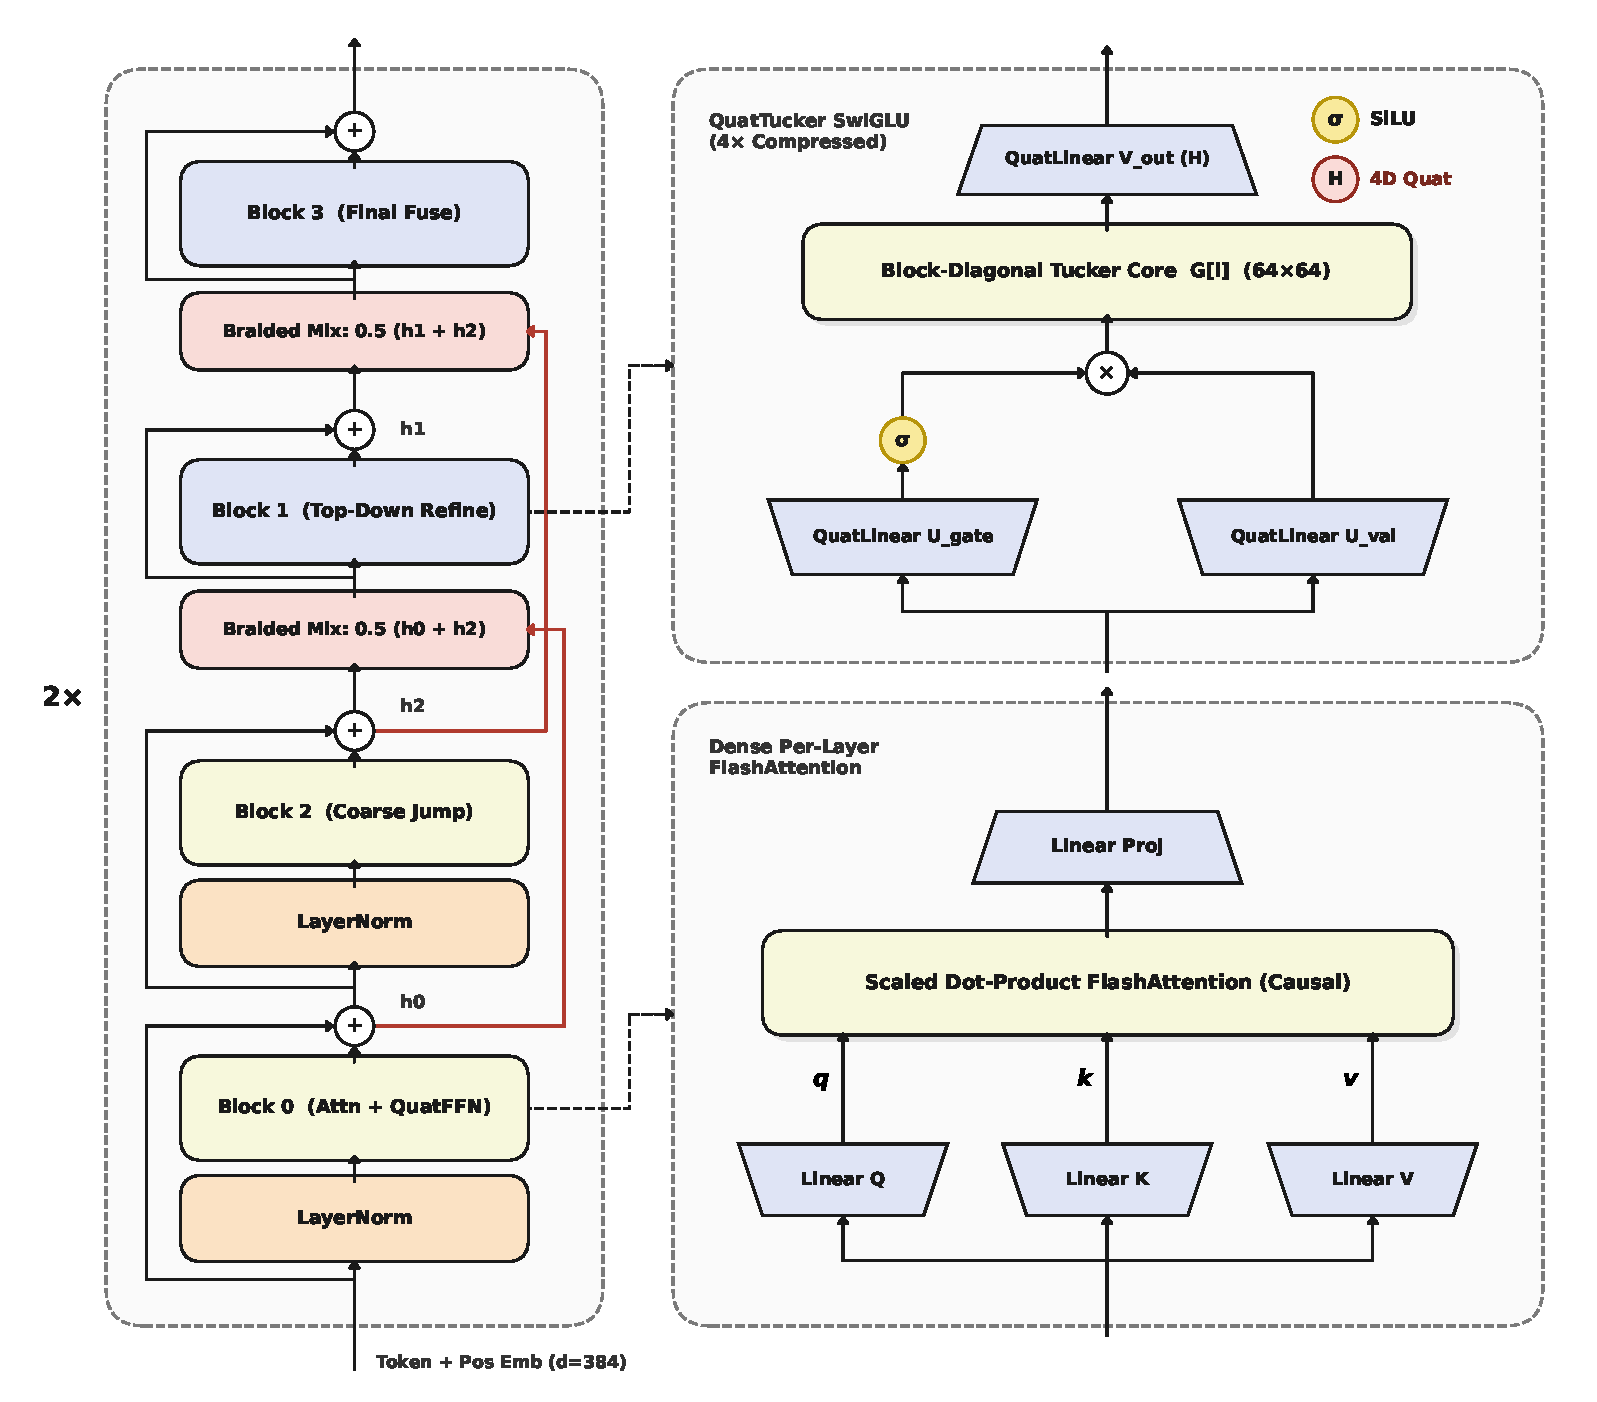
\includegraphics[width=0.78\textwidth]{figures/fig5_architecture_schematic_v2.pdf}
    \caption{\textbf{Overview of QuatTucker-ZigZagGPT-8.} \emph{Left:} Two stacked ($2\times$) Braided \texttt{ZigZag} Diamonds ($0 \to 2 \to 1 \to 3$) routing coarse top-down feedback ($0.5(h_0+h_2)$ and $0.5(h_1+h_2)$) with zero extra FLOPs. \emph{Top-Right:} Shared 4D Quaternion SwiGLU FFN (\texttt{QuatLinear} in $\mathbb{H}$, $4\times$ compressed) modulated by a depth-specific $64 \times 64$ real-valued Block-Diagonal Tucker Core $G[l]$. \emph{Bottom-Right:} Independent dense per-layer \texttt{CausalFlashAttn}.}
    \label{fig:arch}
\end{figure*}

\section{Related Work}
\paragraph{Looped \& Equilibrium Transformers.} Universal Transformers \cite{dehghani2019universal} and ALBERT \cite{lan2020albert} introduced cross-layer weight sharing to decouple parameter count from depth. Deep Equilibrium Models \cite{bai2019deep} generalized this to infinite depth via fixed-point root finding and $O(1)$-memory implicit differentiation. Giannou et al.\ \cite{giannou2023looped} proved that looped transformers can emulate general-purpose programmable computers. Our tensor cuboid formulation generalizes looped networks into \emph{time-inhomogeneous} loops: the shared factor matrices serve as the loop body while tiny depth-specific Tucker cores $G_l$ act as step-specialized instruction pointers.

\paragraph{Tensor Decompositions \& Hypercomplex Networks.} Novikov et al.\ \cite{novikov2015tensorizing} compressed fully connected layers via Tensor-Train decompositions, building on classical CP and Tucker theory \cite{kolda2009tensor}. In NLP, Tay et al.\ \cite{tay2019lightweight} and Parcollet et al.\ \cite{parcollet2019quaternion} demonstrated up to $75\%$ parameter savings using Quaternion algebra ($\mathbb{H}$). We extend this line by combining fused Hamilton GEMMs with SwiGLU gating \cite{shazeer2020glu} and Block-Diagonal Tucker cores specifically tailored for \texttt{bfloat16} \texttt{torch.compile} fusion.

\paragraph{Algorithmic Grokking \& Small-LM Benchmarks.} Power et al.\ \cite{power2022grokking} identified grokking---delayed generalization long after training memorization---on modular arithmetic. Eldan \& Li \cite{eldan2023tinystories} introduced \texttt{TinyStories} to evaluate sub-10M language models, while Penedo et al.\ \cite{penedo2024fineweb} curated \texttt{FineWeb-Edu} as a high-signal modern pretraining benchmark.

\section{Methodology}

\subsection{Annealed Gated Bounce-Back Scaffolding}
Given an $L$-layer network with input projection $x_0$, we introduce a conditional bounce-back gate after intermediate layers $k \in \{2, \dots, L-1\}$ driven by the layer residual $\Delta h_k = h_k - h_{k-1}$:
\begin{equation}
    p_k = \sigma\!\left(w_g^\top \Delta h_k + b_g\right) \in (0, 1).
\end{equation}
During training, the representation is softly blended with a feedback pass through $L_1$:
\begin{equation}
    h_k' = p_k \, L_1(x_0 + \Delta h_k) + (1 - p_k) \, h_k,
\end{equation}
optimized under a sparsity-taxed objective $\mathcal{L} = \mathcal{L}_{\text{task}} + \lambda \frac{1}{K}\sum_k \mathbb{E}[p_k]$. At inference, samples with $p_k \le \tau$ ($\tau=0.5$) hard-skip $L_1$ entirely.

\subsection{Braided ZigZag Diamond Routing}
For any 4-layer block $(\mathcal{B}_0, \mathcal{B}_1, \mathcal{B}_2, \mathcal{B}_3)$, we replace sequential execution with a braided diamond (Figure~\ref{fig:zigzag_routing} and Figure~\ref{fig:arch}, Left):
\begin{align}
    h_0 &= \mathcal{B}_0(x), \qquad h_2 = \mathcal{B}_2(h_0), \\
    h_1 &= \mathcal{B}_1\!\left(\tfrac{1}{2}(h_0 + h_2)\right), \qquad h_3 = \mathcal{B}_3\!\left(\tfrac{1}{2}(h_1 + h_2)\right).
\end{align}
\begin{figure*}[t]
    \centering
    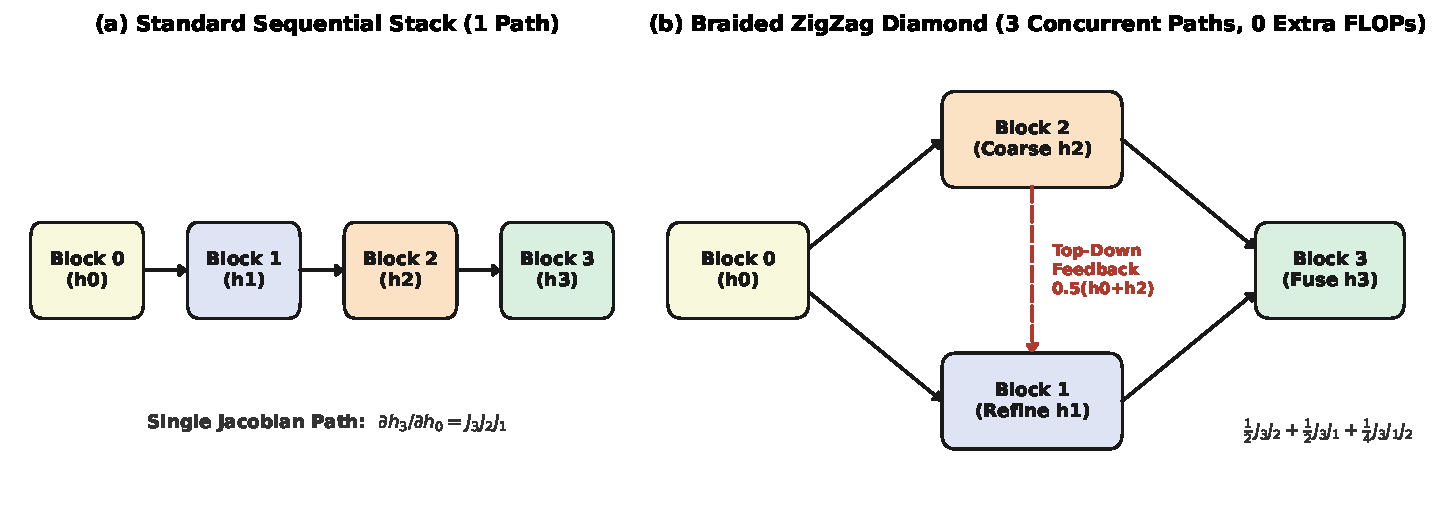
\includegraphics[width=0.92\textwidth]{figures/fig7_zigzag_routing.pdf}
    \caption{\textbf{Braided \texttt{ZigZag} Diamond Routing vs.\ Sequential Stacking.} Reordering execution from $0 \to 1 \to 2 \to 3$ to $0 \to 2 \to 1(0.5(h_0+h_2)) \to 3(0.5(h_1+h_2))$ expands a single Jacobian path into three concurrent gradient pathways with zero extra parameters or FLOPs.}
    \label{fig:zigzag_routing}
\end{figure*}
\begin{proposition}[Multi-Path Gradient Flow]
Let $J_l = \frac{\partial \mathcal{B}_l}{\partial x}$. In a braided \texttt{ZigZag} diamond, the Jacobian $\frac{\partial h_3}{\partial h_0}$ decomposes into three concurrent pathways of lengths $2$, $2$, and $3$ (corresponding to total depths $3$, $3$, and $4$ from $x$):
\begin{equation}
    \frac{\partial h_3}{\partial h_0} = \tfrac{1}{2} J_3 J_2 + \tfrac{1}{2} J_3 J_1 + \tfrac{1}{4} J_3 J_1 J_2,
\end{equation}
providing simultaneous short-range gradient highways and top-down nonlinear refinement at identical FLOPs to sequential stacking.
\end{proposition}

\subsection{CP \& Block-Diagonal Tucker SwiGLU Cuboids}
We treat all $L=4$ FFN layers inside a diamond as a single 3D cuboid $\mathcal{W} \in \mathbb{R}^{4 \times d \times R}$. Rather than storing $4$ independent dense FFNs ($O(4 d R)$), we share a single SwiGLU basis $(U_{\text{gate}}, U_{\text{val}} \in \mathbb{R}^{d \times R}, V_{\text{out}} \in \mathbb{R}^{R \times d})$.

In \textbf{CP-ZigZag}, depth $l$ applies a diagonal eigenvalue vector $A_l \in \mathbb{R}^R$:
\begin{equation}
    \text{FFN}_{\text{CP}}(x, l) = \left(\text{SiLU}(x U_{\text{gate}}) \odot (x U_{\text{val}}) \odot A_l\right) V_{\text{out}}.
\end{equation}
In \textbf{Tucker-ZigZag}, we upgrade diagonal scaling to a real-valued Block-Diagonal Tucker Core $G_l \in \mathbb{R}^{b \times b}$ ($b=64$, $N_b = R/b$ blocks), initialized as $(I_b + 0.05\,\mathcal{N}(0,1)) R^{-1/2}$:
\begin{equation}
    z = \text{SiLU}(x U_{\text{gate}}) \odot (x U_{\text{val}}) \in \mathbb{R}^{B \times T \times R},
\end{equation}
\begin{equation}
    z_{\text{mix}} = \text{flat}\!\left(\text{blk}(z)\, G_l\right) \in \mathbb{R}^{B \times T \times R},
\end{equation}
where $\text{blk}(\cdot)$ reshapes the rank axis into $[N_b, b]$ and $\text{flat}(\cdot)$ restores $[R]$. This allows each depth to perform full $64$-dimensional subspace rotations while remaining $100\%$ native to \texttt{bfloat16} Tensor Cores.

\subsection{4D Quaternion Hamilton GEMM ($\mathbb{H}$)}
In \textbf{QuatTucker-ZigZagGPT}, we parameterize $U_{\text{gate}}, U_{\text{val}}, V_{\text{out}}$ over the quaternion algebra $\mathbb{H}$. For $in\_f = 4 i_q$ and $out\_f = 4 o_q$, we store four real matrices $W_r, W_i, W_j, W_k \in \mathbb{R}^{o_q \times i_q}$ ($4\times$ fewer parameters) and assemble the $4 \times 4$ Hamilton block matrix $W_{\mathbb{H}} \in \mathbb{R}^{4 o_q \times 4 i_q}$:
\begin{equation}
    W_{\mathbb{H}} = \begin{bmatrix}
    W_r & -W_i & -W_j & -W_k \\
    W_i &  W_r & -W_k &  W_j \\
    W_j &  W_k &  W_r & -W_i \\
    W_k & -W_j &  W_i &  W_r
    \end{bmatrix}.
\end{equation}
Computing $y = x W_{\mathbb{H}}^\top$ by materializing $W_{\mathbb{H}}$ once per forward call dispatches a single fused cuBLAS GEMM, achieving identical wall-clock throughput to dense \texttt{bfloat16} linear layers on NVIDIA L4 GPUs.

\section{Empirical Results}

\subsection{8-Bit Parity \& Annealed Scaffolding}
We evaluate 10 architectures on 8-bit Parity (256 bitstrings, 192 train / 64 unseen test, 5 seeds, AdamW \cite{loshchilov2019decoupled} $\text{lr}=3\times 10^{-3}$, $\text{wd}=10^{-2}$, 600 steps). As shown in Figure~\ref{fig:parity}a, \textbf{CP-CuboidNet} achieves $92.2 \pm 7.6\%$ with only $1,522$ parameters ($3.2\times$ smaller than \texttt{ResNet4} \cite{he2016deep} at $70.3 \pm 22.4\%$). Figure~\ref{fig:parity}b reveals a sharp U-shaped self-distillation transition in \texttt{GatedBounce4}: at $\lambda=0.2$, test accuracy peaks at $90.9 \pm 14.3\%$ while inference bounce rate collapses to $0.0\%$.

\begin{figure*}[t]
    \centering
    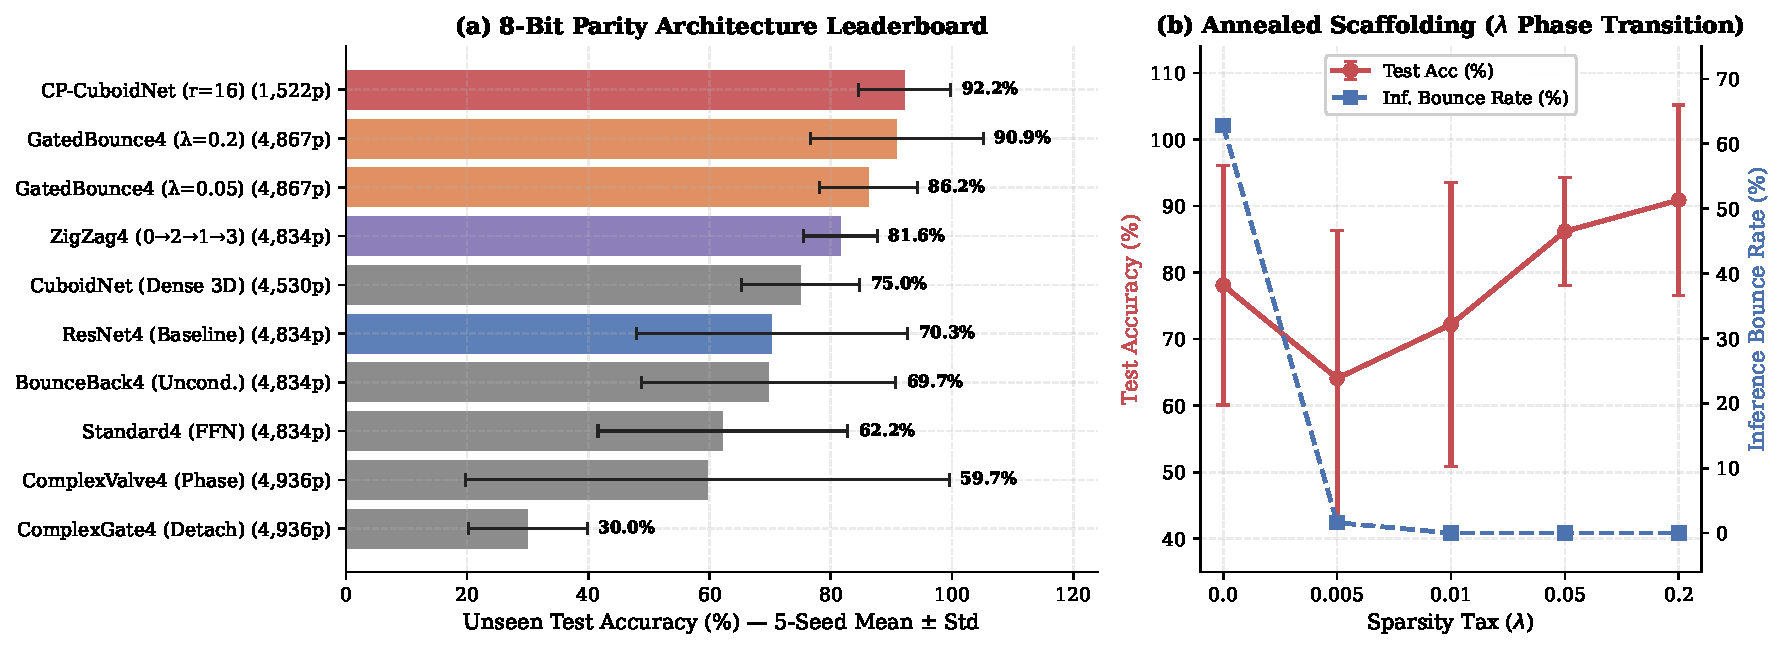
\includegraphics[width=0.96\textwidth]{figures/fig1_parity_and_scaffolding.pdf}
    \caption{\textbf{8-Bit Parity 5-Seed Study.} (a) Architecture leaderboard with $\pm 1\sigma$ error bars and parameter counts. \texttt{CP-CuboidNet} ($1,522$ params) achieves $92.2\%$, outperforming \texttt{ResNet4} by $+21.9\%$ at $3.2\times$ compression. (b) Sparsity tax ($\lambda$) phase transition in \texttt{GatedBounce4}: strong $\lambda=0.2$ forces full self-distillation to $0.0\%$ inference bounce rate.}
    \label{fig:parity}
\end{figure*}

\subsection{Multi-Domain Compression \& Grokking}
We validate \texttt{CP-CuboidNet} across three further domains: (1) 8-layer Mod-53 Addition Grokking ($(a+b)\bmod 53$, 50/50 split, $\text{wd}=1.0$, 1,200 steps), (2) \texttt{sklearn} $8\times 8$ Handwritten Digits (1,797 samples, 80/20 split), and (3) a 3-turn intertwined 2D Double Spiral (1,000 points, 70/30 split). Table~\ref{tab:multidomain} and Figure~\ref{fig:mod53} show consistent $3.1\times$--$7.6\times$ compression. On Mod-53, \texttt{CP-Cuboid-8} ($18,997$ params) climbs monotonically to $100.0\%$ with zero post-grokking slingshot, whereas \texttt{ResNet-8} ($144,373$ params) oscillates back to $88.2\%$.

\begin{table}[h]
\centering
\caption{Multi-Domain \texttt{CP-CuboidNet} vs.\ \texttt{ResNet} Compression.}
\label{tab:multidomain}
\footnotesize\setlength{\tabcolsep}{3.5pt}
\begin{tabular}{@{}lccc@{}}
\toprule
\textbf{Domain} & \textbf{ResNet} & \textbf{CP-Cuboid} & \textbf{Comp.} \\
\midrule
8-Bit Parity (5-seed) & 70.3\% (4.8k) & \textbf{92.2\%} (1.5k) & $3.2\times$ \\
Mod-53 Grokking (8L) & 88.2\% (144k) & \textbf{100.0\%} (19.0k) & $7.6\times$ \\
Handwritten Digits & 98.33\% (22.0k) & 96.94\% (7.1k) & $3.1\times$ \\
3-Turn Double Spiral & 95.67\% (4.6k) & \textbf{96.00\%} (1.3k) & $3.5\times$ \\
\bottomrule
\end{tabular}
\end{table}

\begin{figure}[h]
    \centering
    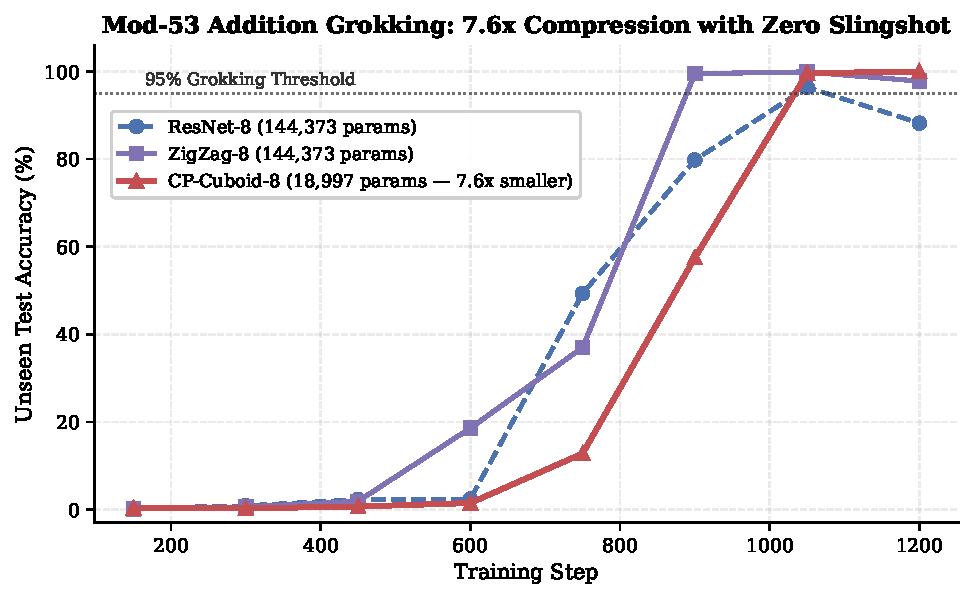
\includegraphics[width=\linewidth]{figures/fig2_mod53_grokking.pdf}
    \caption{\textbf{Mod-53 Addition Grokking (8 Layers).} \texttt{CP-Cuboid-8} ($7.6\times$ smaller) achieves monotonic $100.0\%$ generalization without the post-grokking instability observed in \texttt{ResNet-8}.}
    \label{fig:mod53}
\end{figure}

\subsection{Character-Level Language Modeling (Tesla T4)}
On \texttt{TinyShakespeare} (1.1M chars) and \texttt{TinyStories} (8.7M train / 406k val chars, 2,000 steps), we first optimized T4 GPU execution: replacing software-emulated \texttt{bfloat16} and 4D \texttt{torch.einsum} with native \texttt{float16} + \texttt{GradScaler} and contiguous \texttt{matmul} delivered a \textbf{$13.5\times$ wall-clock speedup} ($813.8\text{s} \to 60.1\text{s}$, Figure~\ref{fig:tinystories}b). Pairing 4 interleaved attention layers with a shared SwiGLU-Cuboid and braided \texttt{ZigZag} routing (\texttt{CP-ZigZagLM}) beat PyTorch's \texttt{StandardTransformer-4} at an exact 1.84M iso-parameter budget ($2.48$ vs.\ $2.54$ PPL, Figure~\ref{fig:tinystories}a).

\begin{figure*}[t]
    \centering
    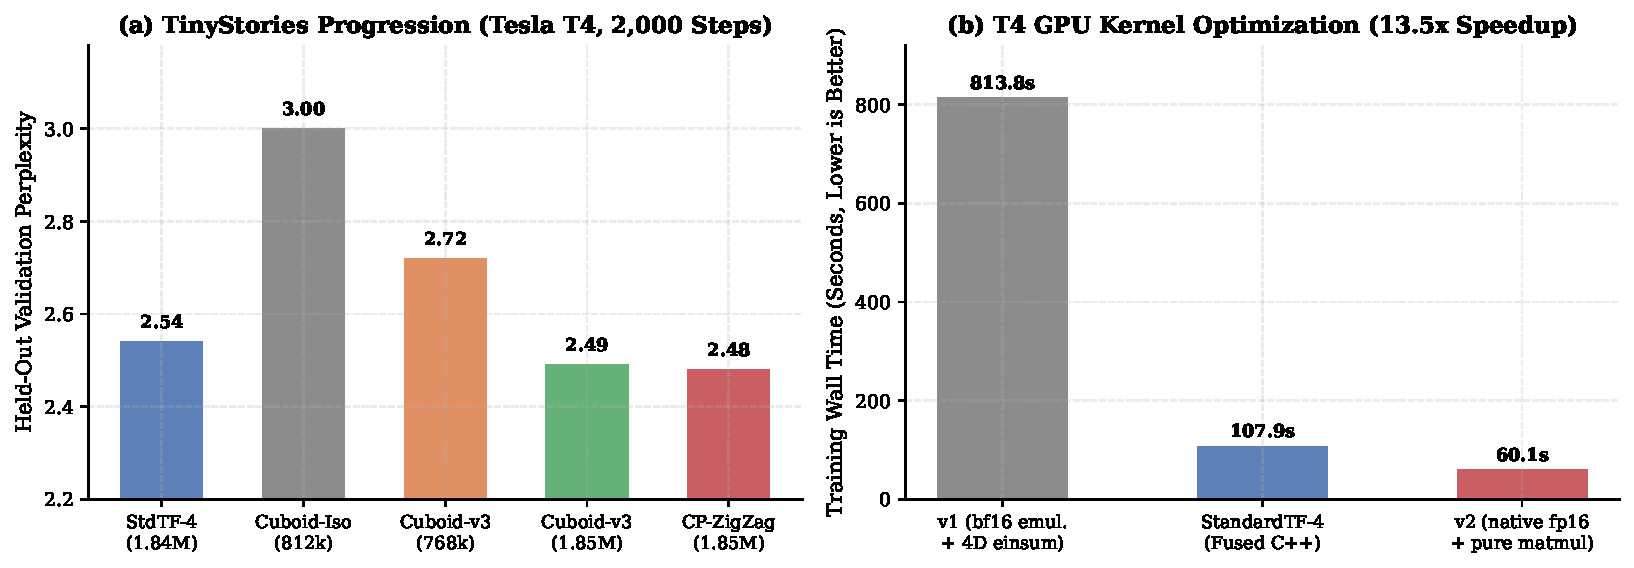
\includegraphics[width=0.95\textwidth]{figures/fig6_tinystories_t4.pdf}
    \caption{\textbf{Tesla T4 GPU Progression.} (a) On 8.7M-char \texttt{TinyStories}, \texttt{CP-ZigZagLM} ($2.48$ PPL) outperforms \texttt{StandardTransformer-4} ($2.54$ PPL) at an exact 1.84M iso-parameter budget. (b) Eliminating emulated \texttt{bf16} and 4D \texttt{einsum} yields a $13.5\times$ speedup on T4 ($813.8\text{s} \to 60.1\text{s}$).}
    \label{fig:tinystories}
\end{figure*}

\subsection{33.5M \texttt{FineWeb-Edu} BPE Pretraining (NVIDIA L4)}
We scale to modern GPT-2 BPE pretraining \cite{radford2019language} ($V=50,257$, 11.4M train / 600k val tokens from \texttt{FineWeb-Edu}, $B=32, T=256$, 3,000 steps, \texttt{bfloat16}, \texttt{torch.compile}, fused AdamW $\text{lr}=10^{-3}$, $\text{wd}=0.1$, cosine schedule, GPT-2 $\sigma=0.02$ embedding init). All models share identical $d=384$ weight-tied embeddings ($19.3\text{M}$ params) and 8 \texttt{CausalFlashAttn} layers.

Figure~\ref{fig:fineweb} presents the complete 12-checkpoint validation trajectories, with key milestones tabulated in Table~\ref{tab:fineweb_full}. \texttt{CP-ZigZagGPT-8} and \texttt{Tucker-ZigZagGPT-8} outperform \texttt{StandardGPT-8} at \textbf{all 12 evaluated checkpoints} with zero crossings, reaching \texttt{StandardGPT-8}'s final step-3,000 loss ($5.2310$) by step 2,250 ($5.1990$)---a \textbf{$25\%$ early token-efficiency gain}. Upgrading to 4D Quaternion elements (\texttt{QuatTucker-ZigZagGPT-8}) cuts the backbone in half ($7.2\text{M}$ vs.\ $14.3\text{M}$) while achieving the best final validation loss (\textbf{5.1339}, \textbf{169.68 PPL}) and maintaining monotonic descent without the step-3,000 validation uptick seen in the 14.3M-backbone baselines (Figure~\ref{fig:backbone}).

\begin{table*}[t]
\centering
\caption{\textbf{\texttt{FineWeb-Edu} GPT-2 BPE Validation Loss Trajectory (NVIDIA L4, 3,000 Steps).} All models share 19.3M token embeddings. \texttt{QuatTucker-ZigZagGPT-8} halves the backbone (7.2M vs.\ 14.3M) and achieves the best final loss (5.1339 / 169.68 PPL).}
\label{tab:fineweb_full}
\footnotesize\setlength{\tabcolsep}{4.5pt}
\begin{tabular}{@{}lccccccccc@{}}
\toprule
\textbf{Model} & \textbf{Total (BB)} & \textbf{250} & \textbf{500} & \textbf{1000} & \textbf{1500} & \textbf{2000} & \textbf{2500} & \textbf{3000 (Final)} & \textbf{Final PPL} \\
\midrule
StandardGPT-8 & 33.5M (14.3M) & 6.6911 & 6.4302 & 5.8940 & 5.5593 & 5.3269 & 5.2596 & 5.2310 & 186.98 \\
CP-ZigZagGPT-8 & 33.6M (14.3M) & 6.6151 & 6.2858 & 5.7718 & 5.4518 & \textbf{5.2628} & 5.1872 & 5.1687 & 175.68 \\
Tucker-ZigZagGPT-8 & 33.6M (14.3M) & \textbf{6.6065} & \textbf{6.2563} & \textbf{5.7645} & 5.4516 & 5.2657 & 5.1826 & 5.1655 & 175.13 \\
\textbf{QuatTucker-ZigZag-8} & \textbf{26.5M (7.2M)} & 6.6461 & 6.2790 & 5.7778 & \textbf{5.4374} & 5.2653 & \textbf{5.1786} & \textbf{5.1339} & \textbf{169.68} \\
\bottomrule
\end{tabular}
\end{table*}

\begin{figure}[h]
    \centering
    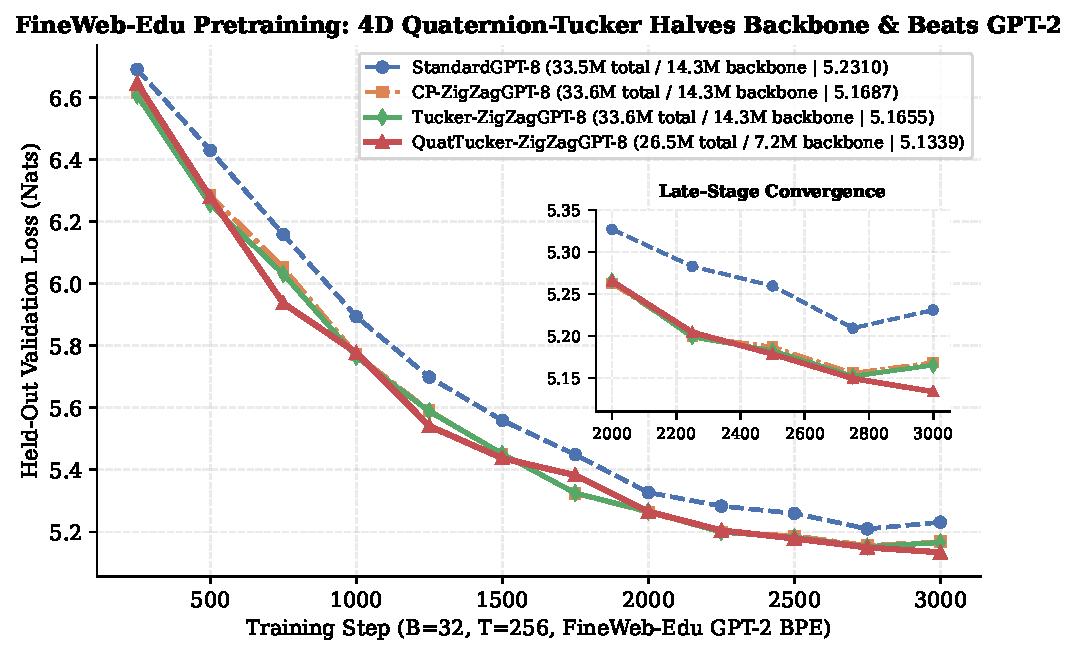
\includegraphics[width=\linewidth]{figures/fig3_fineweb_scaling.pdf}
    \caption{\textbf{\texttt{FineWeb-Edu} Validation Descent (3,000 Steps).} \texttt{QuatTucker-ZigZagGPT-8} (7.2M backbone) achieves monotonic convergence to $5.1339$ loss while all three 14.3M-backbone models tick upward at step 3,000.}
    \label{fig:fineweb}
\end{figure}

\begin{figure}[h]
    \centering
    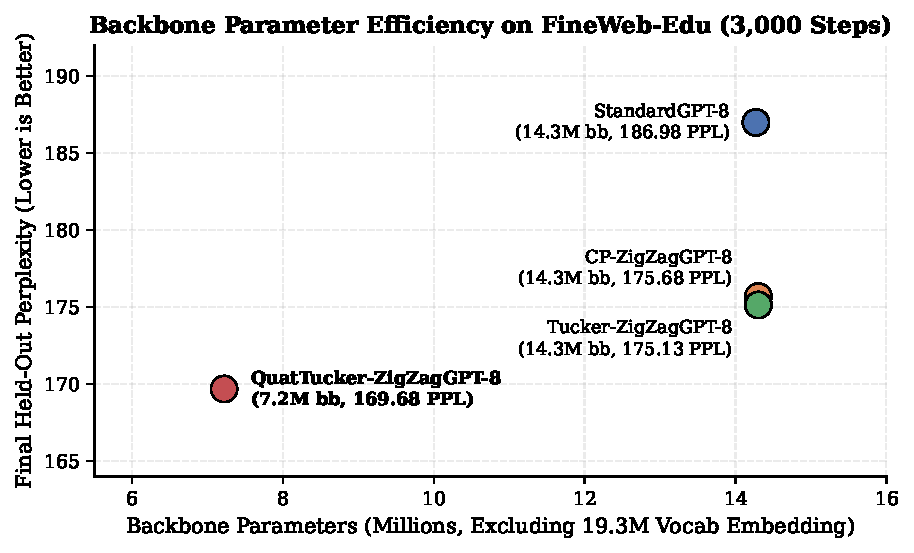
\includegraphics[width=\linewidth]{figures/fig4_backbone_efficiency.pdf}
    \caption{\textbf{Backbone Parameter Efficiency Frontier.} \texttt{QuatTucker-ZigZagGPT-8} shifts the Pareto frontier by halving backbone parameters ($7.2\text{M}$ vs.\ $14.3\text{M}$) while reducing perplexity by $-17.30$ points.}
    \label{fig:backbone}
\end{figure}

\section{Negative Results \& Architectural Laws}
Scientific rigor requires documenting where mechanisms fail. Four ablations established strict design boundaries:
\begin{enumerate}
    \item \textbf{Attention Cannot Be CP-Shared (\texttt{FullTucker-ZigZagGPT-12}):} Sharing CP-decomposed $Q,K,V,O$ projections across 4 depths to stack 12 layers at 32.7M params degraded step-500 validation loss to $6.8358$ (vs.\ $6.2563$ for dense attention). Attention layers require independent per-layer specialization across syntactic distances, whereas FFNs act as shared associative memory banks that thrive under hypercomplex tensor compression.
    \item \textbf{Complex FFT Tucker Cores Break Compiler Fusion:} Replacing real Tucker cores with circulant \texttt{torch.fft.rfft} triggered a \texttt{TorchInductor} fallback for complex operators ($3\times$ slowdown, $131.2\text{s}$ vs.\ $44.1\text{s}$ at step 250) and trailed real-valued Tucker cores ($6.6397$ vs.\ $6.6065$).
    \item \textbf{Periodic Phase-Gated Backprop Valves:} Hard-detaching backprop via unit-circle phase coherence starved early layers ($0.0\%$ backprop, $30.0\%$ parity acc); smooth periodic backward hooks exhibited bimodal phase-wrap instability ($59.7 \pm 39.9\%$).
    \item \textbf{Weight-Tied Embedding Initialization:} Default PyTorch $\sigma=1.0$ embedding init inflated step-1 logits to $\approx 250$, wasting peak cosine LR and costing $1.42$ full validation loss points at step 3,000 ($6.5944$ vs.\ $5.1687$) compared to standard GPT-2 $\sigma=0.02$ initialization.
\end{enumerate}

\section{Limitations \& Future Work}
Our \texttt{FineWeb-Edu} runs trained for 3,000 steps ($\approx 24.6\text{M}$ tokens). While \texttt{QuatTucker-ZigZagGPT-8} showed $25\%$ early token efficiency and $2\times$ backbone compression, verifying this lead at Chinchilla scale (2B--3B tokens, 125M params, RoPE \cite{su2024roformer}, RMSNorm \cite{zhang2019root}) is our immediate next step.

\clearpage
\onecolumn
\raggedbottom
{\small
\bibliography{references}
}
\end{document}
